\chapter{Implementation of Direct GPU-FPGA Communication}
\label{section:implementation}

%GPUDirect RDMA method will be used
In this thesis, a similar approach as described by Susanto \cite{susanto} will be used for the direct GPU-FPGA communication.
The transfer will be handled mainly by the DMA controller on the FPGA.
The CPU will only coordinate the transfer.
On the GPU side the NVIDIA GPUDirect RDMA mechanism is required.


%TODO:
%RDMA theory?
%dataflow inside the fpga, avalon etc
%implementation of the cpu-fpga dma
%kernel-to-user interrupts for dma
%basic rdma implementation only one descriptor at a time
%advanced: merge descriptors, bursts?


\section{Altera PCIe Driver and IP Overview}

%dma controller: dma-write/dma-read
%msgdma diagram
%hard pcie ip, ATT
%cpu-fpga dma?


%TODO: dma descriptor

Altera's OpenCL implementation consists mainly of a dynamic Linux library, a PCIe driver and a \emph{Board Support Package} (BSP) containing the Intellectual Property (IP) cores to be deployed on the FPGA \cite{altera_driver}.
The dynamic library is proprietary but the BSP and the driver are open source and can be analyzed and modified.

The components of the Altera OpenCL IP stack are interconnected by the \emph{Avalon Memory-Mapped} (Avalon-MM) interconnect \cite{altera_driver, avalon}.
Avalon-MM is a multi-master/multi-slave bus.
An address range is assigned to each slave connected to the bus.
The master can then initiate transactions to specific slaves by writing to or reading from the corresponding slave addresses, similarly to memory-mapped I/O on the Linux operating system.

The most important cores for this thesis are the PCIe core, the DMA controller core and the DDR memory interface.
Figure \ref{fig:avalonstack} provides an overview of the connections between them.
When the driver writes to the FPGA's PCIe BAR with some additional offset, the PCIe core forwards the data from its RX port to the Avalon interconnect.
Depending on the offset the message is routed to one of the slaves.
In this specific example, to communicate with the DMA controller, the driver has to write to the address \texttt{0xc800} within the FPGA BAR.

\begin{figure}[htb]
	  \centerline{
		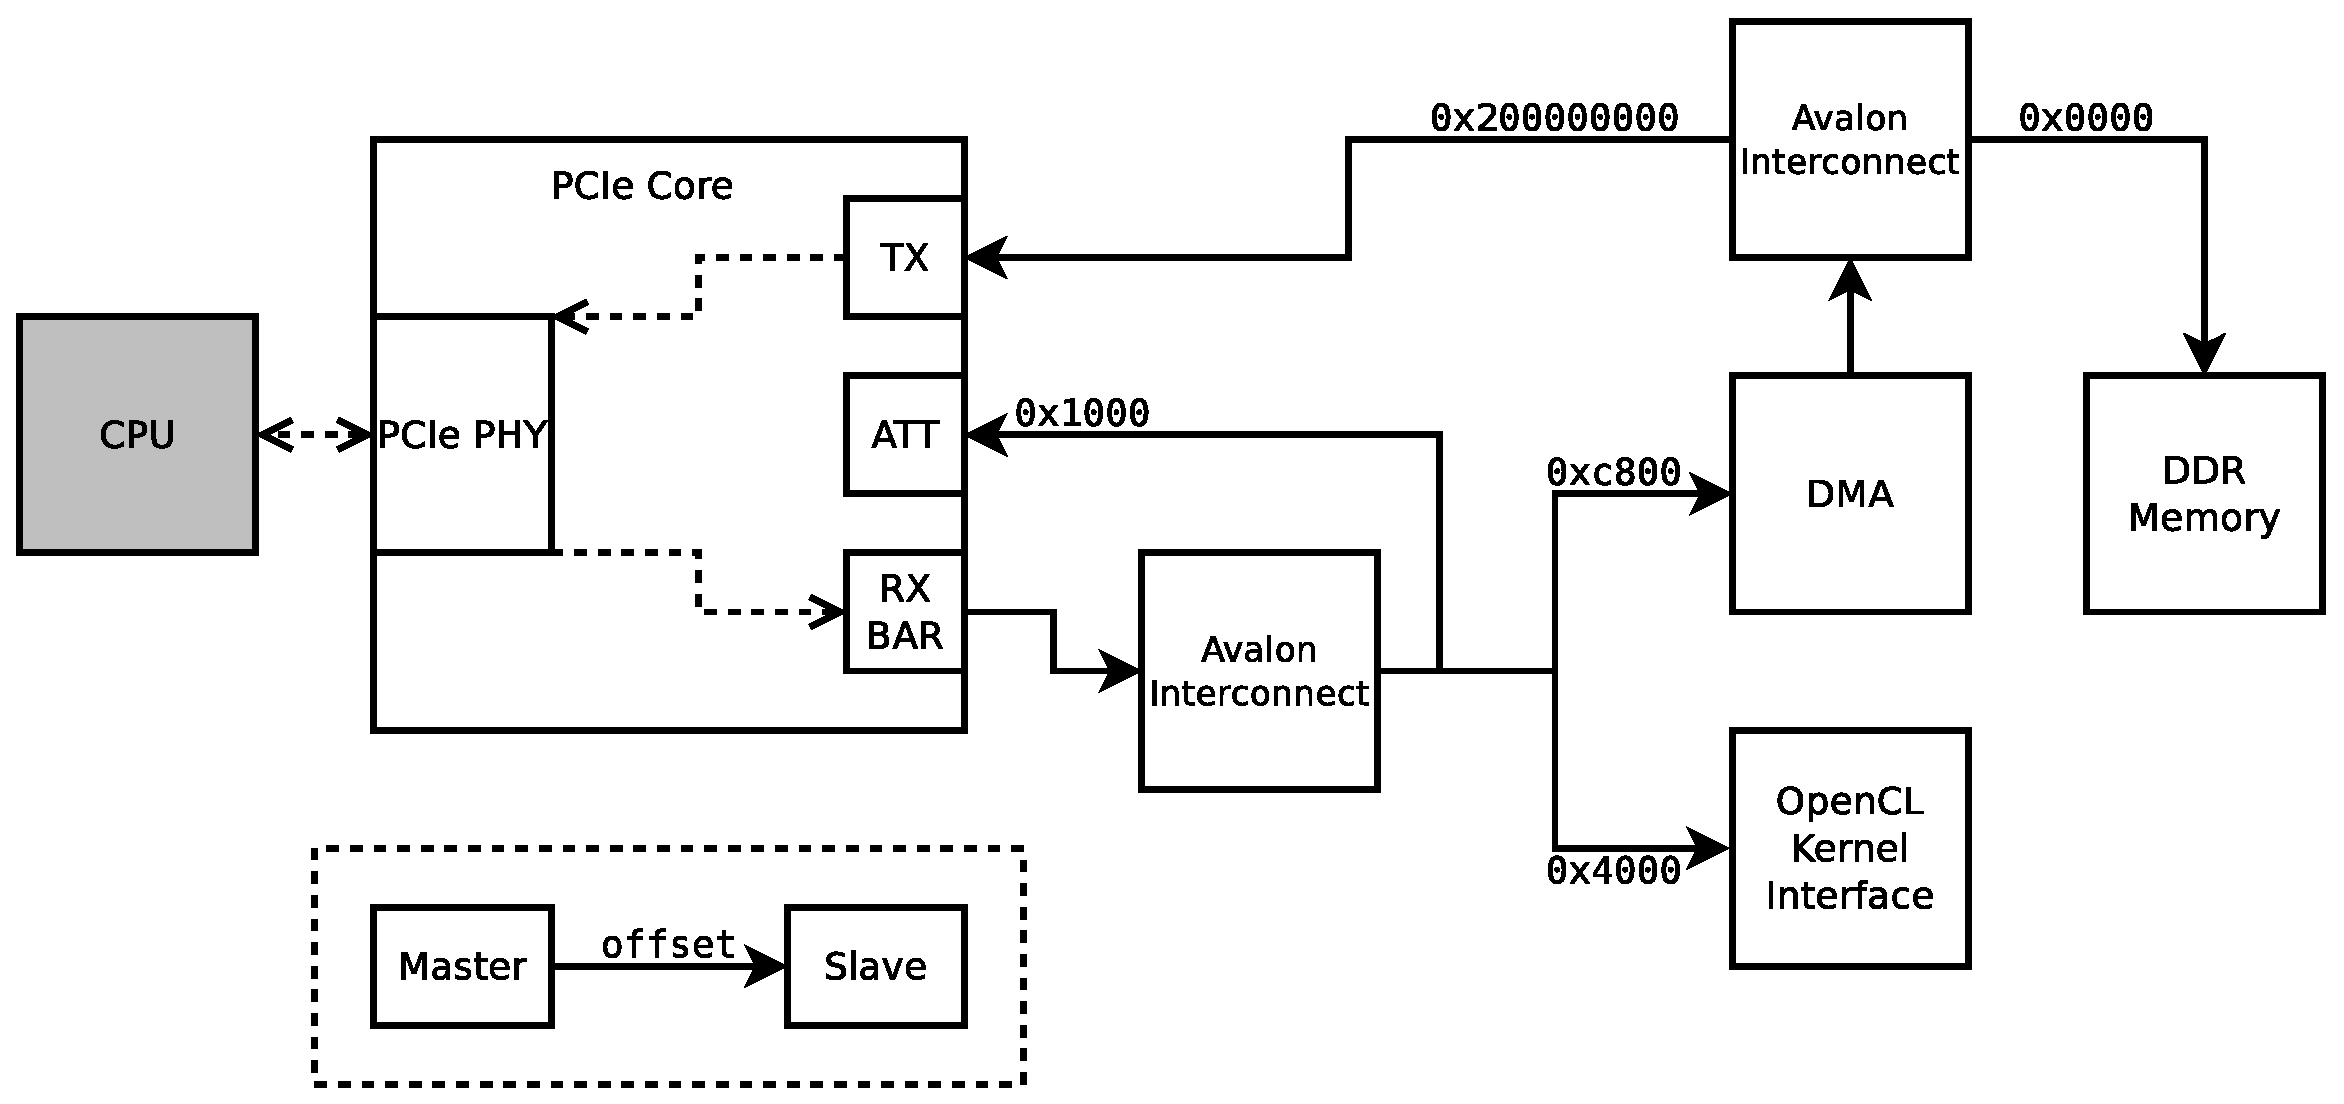
\includegraphics[width=1.1\textwidth]{images/avalonstack2.eps}}
	  \caption{Simplified configuration of the Altera  OpenCL IP stack on the FPGA.
	           Note that the solid arrows represent master/slave relationships and not necessarily the data flow direction.}
	  \label{fig:avalonstack}
\end{figure}


The DMA controller is a \emph{Modular Scatter-Gather DMA} (mSGDMA) IP core \cite{altera_msgdma}.
It is subdivided into a read master, write master and a dispatcher which coordinates the other two components.
A transfer is initiated by writing a 32-byte \emph{descriptor} to the dispatcher.
The descriptor contains all the required information about the desired transfer, including the source and destination memory addresses and the number of bytes to be transmitted.
Then, the dispatcher pushes the descriptors into a FIFO and processes them sequentially.

%descriptor fifo
%control parameter



The PCIe core contains an \emph{Address Translation Table} (ATT) which stores physical PCIe addresses \cite{altera_pcie_core}.
With an ATT, the DMA controller does not need to differentiate between physical addresses or addresses pointing to on-board DDR memory.
Instead, it can simply write the address it received in the descriptor from the device driver to the Avalon master port.
The Avalon interconnect will then route the signals to either the PCIe core or the FPGA memory.
The PCIe core would then select the required physical address from the ATT.
The differentiation has to made by the device driver.
To specify a physical address it has first to store it in the ATT by writing to offset \texttt{0x1000} (plus the ATT row number).
Then it writes to the offset \texttt{0xc800} (the DMA Controller) the address of the PCIe TX port as seen from the DMA. i.e. an offset of \texttt{0x200000000} plus the ATT row number.
Listing \ref{listing:rdma_pcietxs} shows this calculation in a more portable manner with the macros already defined in the Altera PCIe driver code.
%Then it calculates the address as in listing \ref{listing:rdma_pcietxs} and sends it to the DMA controller.



\begin{lstlisting}[label=listing:rdma_pcietxs, caption=Calculation of the PCIe address as seen from the DMA controller]
unsigned long
pcietxs_addr = (size_t)     ACL_PCIE_TX_PORT 
                 | (att_row *   ACL_PCIE_DMA_MAX_ATT_PAGE_SIZE) 
                 | (physical_addr  &  (ACL_PCIE_DMA_MAX_ATT_PAGE_SIZE - 1));
\end{lstlisting}


The direction of the transfer, i.e. whether data is to be read from or written into the FPGA memory, is specified implicitly by the \texttt{read\_address} and \texttt{write\_address} fields of the descriptor similar to listing \ref{listing:rdma_direction}.

\begin{lstlisting}[label=listing:rdma_direction, caption=Selection of the transfer direction ]
if(direction == READING)
{
	//reading from FPGA memory to PCIe bus
	dmadescriptor.read_address     = fpga_address;
	dmadescriptor.write_address    = pcietxs_address;
}
else
{
	//writing to FPGA memory from PCIe bus
	dmadescriptor.read_address     = pcietxs_address;
	dmadescriptor.write_address    = fpga_address;
}
\end{lstlisting}



\section{GPUDirect RDMA Overview}
\label{section:rdmaoverview}

NVIDIA GPUDirect \cite{gpudirect} is a family of technologies for fast data transfers in high performance computing systems with multiple devices.
Its key features include  an accelerated pipeline for video capture devices, storage devices, peer to peer memory access between GPUs and RDMA (Remote Direct Memory Access).
RDMA, as the name implies, is mainly intended to transfer data over network to or from other nodes in a compute cluster.
However it can also be used to transfer data to other third party PCIe devices within the same root complex.
One limitation is that it can only be used for NVIDIA Quadro and Tesla graphics cards.
Furthermore, systems which employ an IOMMU are not compatible.


The main idea behind GPUDirect RDMA is that the GPU can expose a region of its global memory into a PCIe BAR \cite{rdma}.
This can then be used by third party devices to access the memory region directly without the round-trip via the CPU.

Since version 4.0, the CUDA platform, on which NVIDIA's OpenCL implementation is based, uses a memory address management system called \emph{Unified Virtual Addressing} (UVA) \cite{cudaguide, rdma}.
With UVA the GPU memory pages are mapped into the system's virtual address space providing a single address space instead of multiple address spaces, one for the CPU and one for each GPU.
For the CUDA platform this simplifies the programming interface, but on the other hand requires pinning for DMA transfers. 


The NVIDIA device driver provides the function \texttt{nvidia\_p2p\_get\_pages} to pin a GPU memory region \cite{rdma}.
This function must be called from within the kernel space, i.e. from the third party device driver.
It accepts a virtual GPU address and, if the pinning is successful, returns a page table struct containing the physical addresses to each GPU memory page.
The virtual GPU address must be aligned to a 64KB boundary.
The listing \ref{listing:rdma_pinning} provides an example of this process.
\texttt{nvidia\_p2p\_put\_pages} is the corresponding function to unpin the pages.
Additionally, a callback function has to be registered which has to call the function \texttt{nvidia\_p2p\_free\_page\_table} to release resources.
This callback is invoked by the NVIDIA driver when it has to revoke the mapping for some reason.
This is mostly the case when the associated user process terminates.


\begin{lstlisting}[label=listing:rdma_pinning, caption=Pinning GPU memory \cite{rdma}, morekeywords={nvidia_p2p_get_pages}]
// do proper alignment, as required by NVIDIA kernel driver 
u64 virt_start = ((u64)address) & GPU_BOUND_MASK;
u64 pin_size   = ((u64)address) + size - virt_start;

struct nvidia_p2p_page_table page_table;
nvidia_p2p_get_pages( 0, 0, virt_start, pin_size, 
                             &page_table, free_callback, &page_table ); 
\end{lstlisting}

For Kepler class GPUs the pages typically have a size of 64KB.
The PCIe BAR is up to 256MB large of which 32MB are reserved for internal use.
This means that, in theory, up to 224MB can be pinned at a time \cite{rdma}.
However, during development, this number has been found to be slightly smaller, around 200MB.

\section{Extension of the Altera PCIe Driver}

%TODO: how does the OpenCL lib interact with the driver?
%separated RDMA and original DMA

The DMA component of the PCIe device driver provided by Altera expects a virtual address that maps to the CPU memory.
It tries to pin the buffer with the \texttt{get\_user\_pages} function to get a list of the pages and their physical addresses.
Simply passing a GPU address to the module will thus result in an error.
Neither will it work by just replacing \texttt{get\_user\_pages} with  \texttt{nvidia\_p2p\_get\_pages}, the corresponding GPU memory pinning function, due to assumptions related to the address space (for example about the page size) and differences in the pinning work flow.
A new RDMA component, managing only the direct GPU-FPGA communication, will thus extend the driver.
Transfers to and from CPU memory will be handled by the original code which shall remain untouched as far as possible.

%
New driver commands \texttt{ACLPCI\_CMD\_RDMA} and \texttt{ACLPCI\_CMD\_RDMA\_UPDATE} are added to differentiate between the original DMA and the new RDMA transfers.
They are issued via file I/O to the \texttt{/dev/acl0} device file, the same way as the original commands.
%TODO? \texttt{aclpci\_rw}
Section \ref{section:userspace} describes in detail how to use the new commands from user space.



\subsection{Basic Version}
%interrupts override
%new commands

%caveats: have to update the original aclpci struct to not confuse the original dma module
%e.g. dma_data.m_old_done_count inside the interrupt handler


%describe why basic version first

To avoid unnecessary complications during development only a very basic RDMA mechanism has been implemented first.
Its limitations include:
\begin{itemize}
	
\item Only one active transfer at a time
\item Only one active descriptor at a time. The next descriptor is sent only after the previous one is finished.
\item The size of descriptors fixed to 4KB. This is equivalent to the maximum size of an ATT entry.
\item Overall transfer size limited to 192MB. As noted in section \ref{section:rdmaoverview} this is roughly the maximum that can be pinned at a time.
\end{itemize}
Section \ref{sec:optimizations} provides an overview over some improvements to this version.

The new RDMA component consists of five main functions. Figure \ref{fig:driver_functions} illustrates their relationship. Their semantics are as follows:


\begin{figure}[htb]
	  \centerline{
		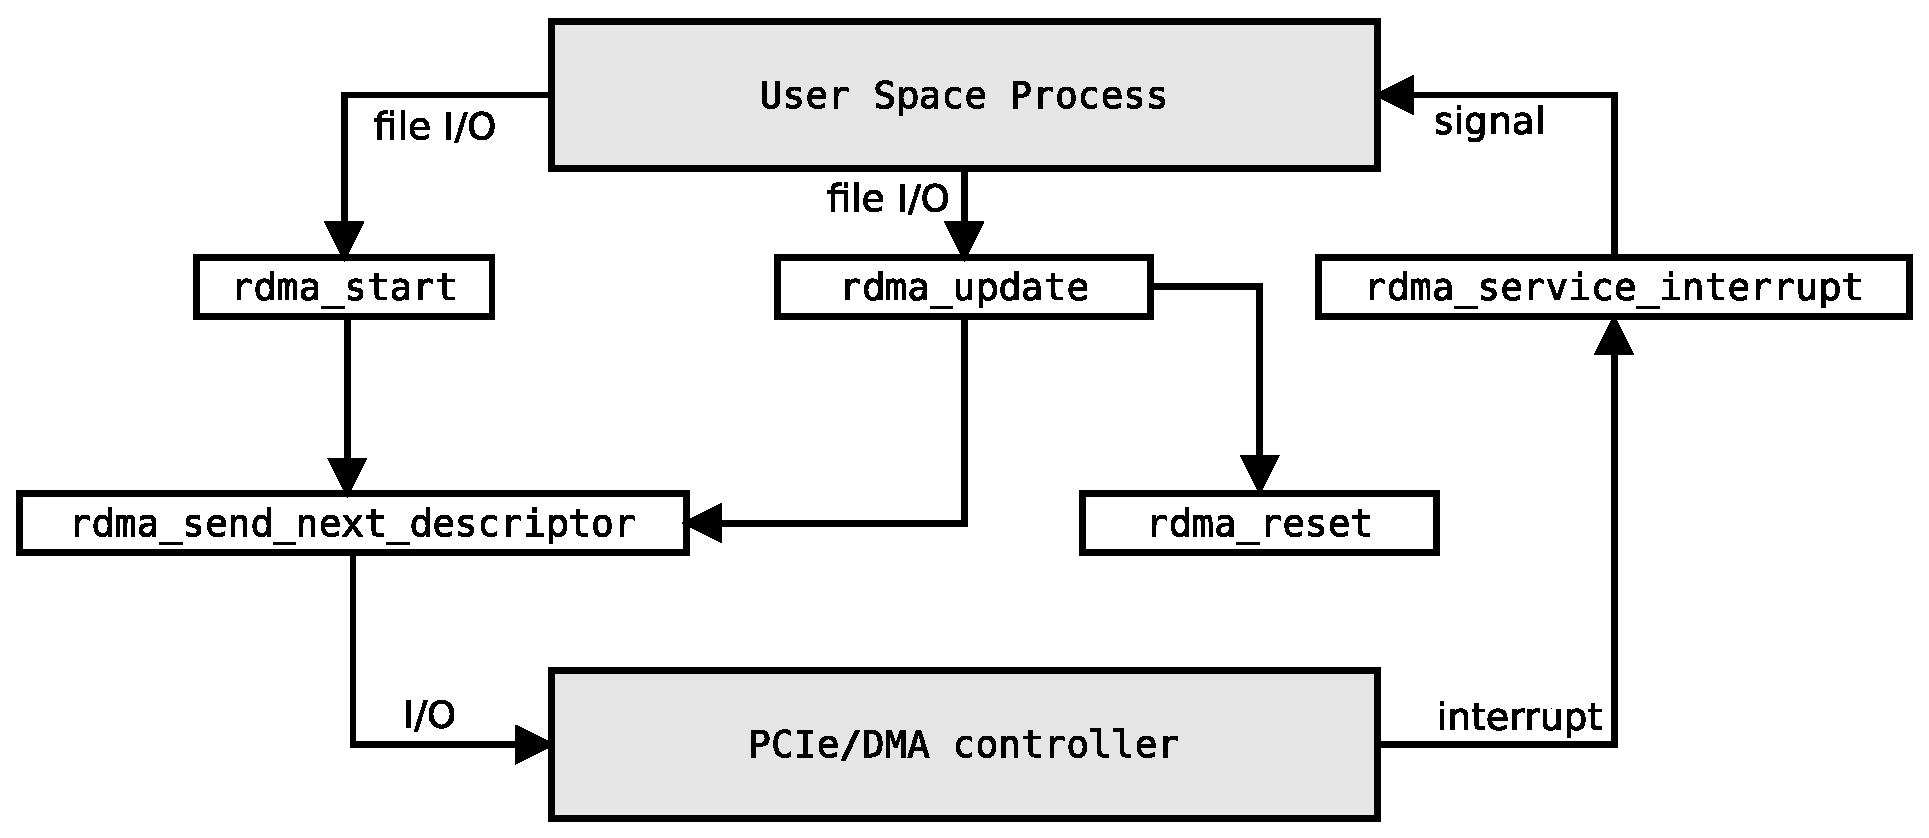
\includegraphics[width=1.0\textwidth]{images/driver_functions.eps}}
	  \caption{The main functions of the new RDMA component}
	  \label{fig:driver_functions}
\end{figure}



%TODO? no state stored between transfers? transfers independent of each other

\begin{list}{$\triangleright$}{\leftmargin=1.0em \itemindent=0em}
%\begin{itemize}
	\item {\bf \texttt{rdma\_start}}: The entry point for all RDMA transfers, invoked when the user space program issues the new \texttt{ACLPCI\_CMD\_RDMA} driver command.
	If there is no other active RDMA transfer, it tries to pin the supplied virtual GPU address as in listing \ref{listing:rdma_pinning}.
	If successful, the actual transfer is started by calling the \texttt{rdma\_send\_next\_descriptor} function.
	
	%TODO: not just  'tries to pin', calls kmd_pin...(), und diese funktion in listing
	%TODO: außerdem diagram updaten
	
	
	\item {\bf \texttt{rdma\_send\_next\_descriptor}}:
	This function performs the actual communication with the DMA controller on the FPGA.
	%TODO: %FIXME: It sets one ATT entry, sets up the dma descriptor
	%TODO: ... as described in section altera pcie overview
	It has to write the physical GPU address to an ATT entry of the PCI core and send a descriptor with the addresses and the size of the transfer.
	After this function, the driver terminates the execution and returns the control to the user space.
	



	
	
	\item {\bf \texttt{rdma\_update}}: This function is invoked from user space with the new driver command \texttt{ACLPCI\_CMD\_RDMA\_UPDATE} to continue with the transfer.
	If the previous descriptor has finished, it calls \texttt{rdma\_send\_next\_descriptor} to send the next one.
	It returns \texttt{1} if there is still data remaining to be transferred and \texttt{0} when the transfer finished to inform the user program.
	%TODO
	
	
	
	\item {\bf \texttt{rdma\_service\_interrupt}}: This is the new DMA interrupt handler for the device driver.
	It replaces the previous interrupt handler \texttt{aclpci\_dma\_service\_interrupt} from the original DMA code.
	It is called whenever the DMA controller signals an interrupt, i.e. when a descriptor is finished.
	Its first task is to acknowledge the interrupt by clearing the IRQ bit as soon as possible, to avoid multiple interrupts in a row.
	An interrupt does not differentiate whether a descriptor is from the RDMA or the original DMA component.
	Therefore the new handler has to relay to the original one if no RDMA transfer is active.
	
	%To avoid that the interupt handler from the original DMA module receives interrupts that are intended

\begin{lstlisting}[label=listing:rdma_clear_irq, caption=Acknowledging the interrupt and relaying to the original handler if needed]
// Clear the IRQ bit
dma_write32 (aclpci, DMA_CSR_STATUS, ACL_PCIE_GET_BIT(DMA_STATUS_IRQ) );

//check whether the interrupt is for RDMA or DMA
if( !rdma_active )
{
	//this is an interrupt for the original DMA component
	return( aclpci_dma_service_interrupt( aclpci ) );
}
\end{lstlisting}

An interrupt handler has to return as fast as possible. %TODO: cite (bookmark?)
	Therefore it should not directly call \texttt{rdma\_update} to continue with the transfer.
	Instead, it issues the new \texttt{SIG\_INT\_RDMA} signal to the user process, which in turn drives the transfer with the \texttt{rdma\_update} function.
%TODO: listing of how to send a signal?

At this point, one of the few interactions to the driver's original DMA component has to be made:
this component keeps track of the number of completed descriptors to be able to calculate how much data has been transferred.
This value has to be kept updated, otherwise it will not function correctly.
This update procedure is shown in listing \ref{listing:rdma_done_count}.

\begin{lstlisting}[label=listing:rdma_done_count, caption=Updating the number of completed descriptors in the original code, morekeywords={m_old_done_count}]
// Read the DMA status register
dma_status = dma_read32 (aclpci, DMA_CSR_STATUS );
// Compute how many descriptors completed since last reset
done_count = ACL_PCIE_READ_BIT_RANGE(dma_status, 
                                                 DMA_STATUS_COUNT_HI,
                                                 DMA_STATUS_COUNT_LO );
//have to update the dma_data struct
//so that the original DMA module does not get confused
aclpci->dma_data.m_old_done_count = done_count;
\end{lstlisting}



	
	\item {\bf \texttt{rdma\_reset}}: Unpins the GPU buffer and removes the \texttt{rdma\_active} flag again, so that future hardware interrupts are relayed to the original DMA component.
\end{list}
%\end{itemize}










\subsection{Optimizations}

\label{sec:optimizations}

The version presented above describes only a very basic implementation with the purpose to prevent errors and to be intuitive to understand.
Maximal bandwidth should not be expected from it.
This section presents three main optimizations for higher performance.



\subsubsection*{Larger Descriptor Sizes}

Descriptors of size 4KB, as used above, are convenient because this corresponds to the maximal size of an ATT page.
By increasing the descriptor size, overall less descriptors are required to complete a transfer.
This in turn, reduces the number of interrupts and the delays caused by the software to react to a hardware interrupt.
Larger descriptors can be constructed by simply incrementing the \texttt{bytes} count register sent to the DMA controller.
After the transfer of the first 4KB of an ATT entry is finished, the consecutive ATT entry is used.
However the addresses have to be continuous.
Up to 128 ATT entries can be covered by one descriptor \cite{altera_driver}.
This corresponds to a size of up to 512KB.


\begin{lstlisting}[label=rdma_send_many, caption=Setting the size of a descriptor as large as possible]
for( i=0; i < ACL_PCIE_DMA_MAX_ATT_PER_DESCRIPTOR; i++ )
{
	unsigned offset_i = i * ACL_PCIE_DMA_MAX_ATT_PAGE_SIZE;
	unsigned page_nr_i = offset_i / GPU_PAGE_SIZE;
	
	//check whether the transfer size has already been reached
	if( bytes_sent + dmadesc.bytes >= transfer_size )
	{ break; }
	
	//check whether the next gpu page is consecutive to previous one
	if( page_table->pages[page_nr + page_nr_i]->physical_address 
	     != phymem+page_nr_i * GPU_PAGE_SIZE )
	{ break; }
	
	set_att_entry( aclpci, phymem + offset_i, next_free_att_row );
	dmadesc.bytes += ACL_PCIE_DMA_MAX_ATT_PAGE_SIZE;
	next_free_att_row = (next_free_att_row+1)%ACL_PCIE_DMA_MAX_ATT_SIZE;
}
\end{lstlisting}








\subsubsection*{Multiple Descriptors}

Additionally to larger descriptors, the DMA controller on the FPGA also accepts multiple descriptors at once.
They are buffered in a FIFO queue and processed one after the other.
As with the optimization above, this can reduce the number of delays from an interrupt until the next descriptor.
The size of the FIFO queue is fixed in the hardware to a maximum of 128 descriptors \cite{altera_driver}.
However, the actual number depends even more on the size of the ATT which is limited to 256 entries or 1MB.
Only two 512KB descriptors already span the whole table.
Sending a third one would require to overwrite the ATT entries of the first descriptor which would result in incorrectly transmitted data.

Instead of calling \texttt{rdma\_send\_next\_descriptor} directly, the functions \texttt{rdma\_update} and \texttt{rdma\_start} will now call the new function \texttt{rdma\_send\_many\_descriptors}.

\begin{lstlisting}[label=rdma_send_many, caption=Sending as many descriptors as possible or needed]
//maximum of two descriptors because this would override ATT
for( i = 0; i < 2; i++ )
{
	//check whether all data has been sent already
	if(bytes_sent >= transfer_size){ break; }
	rdma_send_next_descriptor();
}
\end{lstlisting}

Since the descriptors may be of different sizes, two additional values have to be stored between the transfers:
The number of descriptors sent to the FPGA which is incremented in \texttt{rdma\_send\_next\_descriptor} and the number of completed descriptors, updated in the interrupt handler.
Due to possible race conditions, the number of sent descriptors cannot be accessed in the asynchronous interrupt handler: an interrupt may arrive while the driver is still busy sending new descriptors to the DMA controller and thus incrementing this value.
Access synchronization with mutexes or semaphores is not possible because an interrupt handler is not allowed to wait.
The handler will only update the done count to the value read out from the DMA status register.
The \texttt{rdma\_update} function which is called via a command from the user space will then compare those two values.
If equal, then the next descriptors can be issued to the DMA controller.




\subsubsection*{Lazy Unpinning}
\label{section:lazy}

\emph{Lazy Unpinning} is an optimization technique that is recommended by NVIDIA in the GPUDirect RDMA documentation \cite{rdma}.
Pinning GPU memory pages with the function \texttt{nvidia\_p2p\_get\_pages} is an expensive operation that may take several milliseconds to complete.
It should be performed as rarely as possible.
A naive implementation, as the one described above, that pins a buffer before every transfer and unpins it afterwards will not perform to full potential.

For a higher degree of performance, the memory region should be kept pinned after the transfer is finished.
For the first transfer to or from a buffer, the driver still has to pin the memory and the optimization will not affect it.
All following transfers however, will benefit.

To realize this behavior, a look-up table will store the virtual GPU addresses and the corresponding page tables containing the physical addresses between the transfers.
The size of the look-up table is fixed to 6.
Section \ref{section:userspace} explains why this number was chosen.
When a transfer command is initiated, the requested virtual GPU address has to be looked up in the table first.
Actual pinning is then only required if the table does not contain this address.

A buffer should be only unpinned when the table is full to make room for a new entry.
The decision which entry to remove is not straightforward.
A strategy like \emph{least recently used} (LRU) can be beneficial if many buffers (more than 6) have to be accessed in a non-sequential order.
On the other hand, if the access is strictly consecutive it is better to remove always one specific entry and leave the other 5 pinned.
This strategy was selected also because it is beneficial for very large transfers ($>$200MB) and easier to implement.
In future, if a higher degree of control is desired, it may be reasonable to leave this decision to the user application.


When the user space process terminates, the NVIDIA driver revokes the mapping. The look-up table has to be cleaned up accordingly in the callback function.

The look-up table also indirectly removes the limitation of the maximum transfer size of 192MB.
This is explained in section \ref{section:userspace}.
%TODO: this also removes the limitation of 192MB per transfer








\section{GPUDirect RDMA for OpenCL}
\label{section:cl_rdma}

The GPUDirect RDMA technology that allows direct PCIe communication between a NVIDIA GPU and a third-party device is only suppported for the CUDA toolkit and not for OpenCL \cite{rdma}.
The central function \texttt{nvidia\_p2p\_get\_pages} returns the error code \texttt{-EINVAL} if it is called with an address from a buffer allocated by OpenCL.
This thesis proves that it is nevertheless possible to make it work with OpenCL despite the lack of official support.
This section documents the actions that were taken to achieve this.
In subsection \ref{section:reverse}, the communication calls to the NVIDIA driver from the CUDA and OpenCL libraries are analyzed using reverse engineering techniques.
Subsection \ref{section:nvidiamod} describes the modifications to the NVIDIA kernel module that are necessary to imitate CUDA buffer allocation from within OpenCL.



\subsection{Reverse Engineering the NVIDIA Driver Communication}
\label{section:reverse}

%TODO: parts of the assumptions/conclusions are speculative and based on observations from the data/messages

%TODO: in klammern libOpenCL.so libcuda.so  ?? oä
The CUDA and OpenCL dynamic libraries, as provided by NVIDIA, communicate with the NVIDIA kernel module via the \texttt{ioctl} system call \cite{nvidia_driver}.
The \texttt{ioctl} call takes 3 arguments \cite{ioctl}:
\begin{itemize}
	\item an open file descriptor (in this case referring to \texttt{/dev/nvidia0})
	\item a 32-bit request code of which bits 7 to 0 are the \emph{command} number.
		\item a pointer to a parameter stored in the user address space. Its size is encoded in the bits 29 to 16 of the request code mentioned above.
\end{itemize}
Inside the module, the function \texttt{nvidia\_ioctl(...)} is registered as a callback function for this kind of calls.
Besides thread synchronization and several sanity checks the function itself only performs very simple operations like returning device information or the driver version.
For all other commands it relays the \texttt{ioctl} parameters to the \texttt{rm\_ioctl(...)} function which is defined in the  proprietary binary driver.
The semantics of the \texttt{ioctl} commands are not documented by the vendor.

\begin{figure}[htb]
	  \centerline{
		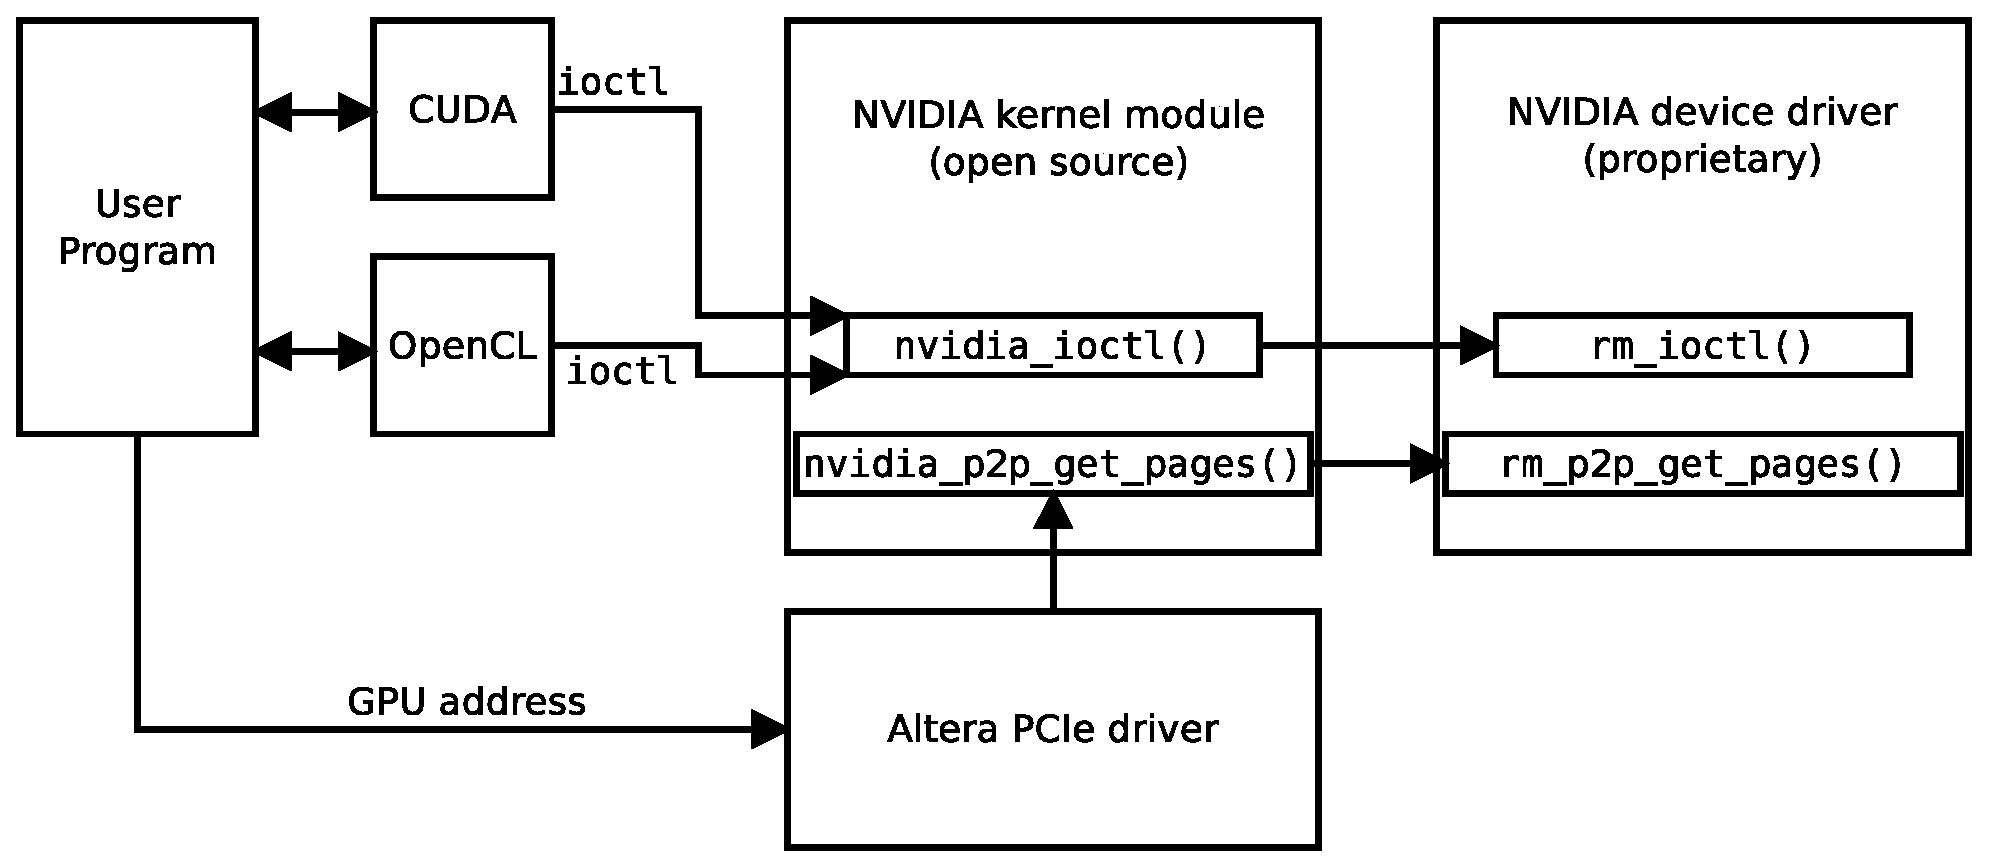
\includegraphics[width=0.9\textwidth]{images/ioctl_com.eps}}
	  \caption{Communication between CUDA/OpenCL and the NVIDIA driver}
	  \label{fig:ioctl_com}
\end{figure}


The GPUDirect RDMA function \texttt{nvidia\_p2p\_get\_pages} is defined in the NVIDIA kernel module and thus has itself no way of knowing whether CUDA or OpenCL is used in the user program.
As a consequence, there must be some differences in the way the two libraries communicate with the module.
Of special interest are the commands for buffer allocation.

%blackbox behaviour

In several experiments, the module has been modified to save all incoming \texttt{ioctl} commands and their parameter data to files on the hard drive to analyze them later.
Two minimalistic applications, one for CUDA and one for OpenCL, that perform as little initialization as needed and allocate one or more memory buffers provided the stimuli.
The data files were then compared for differences.

Some observations from the resulting data are that both libraries perform internal device memory management to some degree.
Small buffer allocations up to a size of 1MB are sometimes not relayed to the driver.
Additionally, NVIDIA's OpenCL implementation seems to utilize lazy buffer allocation, i.e. no communication to the driver happens until the buffer is actually used.
To circumvent this, at least one byte of data had to be written to the buffer for the experiments.

%TODO: in opencl: has to write at least a byte into the buffer
%175 ioctls just for init

The key finding from these experiments is that CUDA sends 3 \texttt{ioctl} messages to the kernel module to allocate a buffer, OpenCL on the other hand sends only 2.
Their request codes are as follows (command numbers highlighted):


\begin{center}
\begin{tabular}{| c | c | c |}
	\hline
	Order & CUDA & OpenCL\\
	\hline
	\hline
	1 & \texttt{0xc0a046{\bf\texttt4a}} &   \texttt{0xc0a046{\bf\texttt4a}}\\
	2 & \texttt{0xc03846{\bf\texttt57}} &   \texttt{0xc03846{\bf\texttt57}}\\
	3 & \texttt{0xc02046{\bf\texttt2a}} &    -\\
	\hline  
\end{tabular}
\end{center}



\emph{Libcudest} \cite{libcudest} is a project aimed at reverse engineering the CUDA platform.
Its documentation pages provide explanations to some of the command codes.
The \texttt{0x4a} and \texttt{0x57} commands are not listed but
the \texttt{0x2a} command, that is missing in OpenCL, is described there as a \emph{GPU method invocation}.
The \texttt{ioctl} parameter is 32 (\texttt{0x20}) bytes large and specifies the GPU method type in the second and third words, an address to the GPU method parameter in the fifth and sixth words and its size in the seventh and eighth words.
No information about the first word of the parameter is provided there.
The analysis of the data from several experiment trials showed that this word always contains the value \texttt{0xc1d00001} for the first process that is started after the NVIDIA driver is loaded.
It is then incremented for each following process that uses CUDA or OpenCL.
Therefore this word will be called \emph{User Identifier} in this thesis.
The following table provides an example of the \texttt{0x2a} \texttt{ioctl} parameter that is missing in OpenCL:

\begin{center}
\begin{tabular}{| c | c | l |}
	\hline
	%\multicolumn{2}{|c|}{parameter of \texttt{0x2a ioctl} command}\\
	Offset & Content & Description \\
	\hline
	\hline
	\texttt{0x00} & \texttt{0xc1d00001} &  \emph{User / Process Identifier} \\
	\hline
	\texttt{0x04} & \texttt{0x5c000007} &  GPU method type \cite{libcudest}\\
	\texttt{0x08} & \texttt{0x503c0104} &  \\
	\hline  
	\texttt{0x0c} & \texttt{0x00000000} &  unknown / always zero\\
	\hline
	\texttt{0x10} & \texttt{0xcbfe9bc0} &  Address to a GPU method parameter \cite{libcudest}\\
	\texttt{0x14} & \texttt{0x00007fff} &  (user space)\\
	\hline
	\texttt{0x18} & \texttt{0x00000004} &  Size of the GPU method parameter \cite{libcudest}\\
	\texttt{0x1c} & \texttt{0x00000000} &  (4 bytes)\\
	\hline
\end{tabular}
\end{center}

This GPU method (\texttt{0x5c000007:503c0104}) is not documented by Libcudest.
The GPU method parameter in this case is 4 bytes large.
Again, after data analysis it has been observed that, similarly to the User Identifier, this parameter value starts with a fixed number for the first device buffer allocation within a process and increments for each of the following buffer allocations.
It will be called \emph{Buffer Identifier} from now on.
For completeness, a GPU method parameter of the first user buffer allocated in CUDA is shown in this table:
\begin{center}
\begin{tabular}{| c | c | l |}
	\hline
	Offset & Content & Description \\
	\hline
	\hline
	\texttt{0x00} & \texttt{0x5c000029} & \emph{Buffer Identifier} \\
	\hline
\end{tabular}
\end{center}

%strace?

Both, the User Identifier as well as the Buffer Identifier are also present in the parameters of the preceding \texttt{0x4a} and \texttt{0x57} \texttt{ioctl} commands (also in OpenCL).
The following table shows a partial example of the \texttt{0x57} command parameter.
The identifiers are located at offsets \texttt{0x00} and \texttt{0x0c}.



\begin{center}
\begin{tabular}{| c | c | l |}
	\hline
	Offset & Content & Description \\
	\hline
	\hline
	\texttt{0x00} & \texttt{0xc1d00001} & \emph{User Identifier} \\
	\hline
	\texttt{0x04} & \texttt{0x5c000001} & {unknown} \\
	\hline
	\texttt{0x08} & \texttt{0x5c000003} & {unknown} \\
	\hline
	\texttt{0x0c} & \texttt{0x5c000029} & \emph{Buffer Identifier} \\
	\hline
	\texttt{0x10} & \texttt{0x00000000} & {unknown} \\
	\hline
	\texttt{0x14} & \texttt{0x00000000} & {unknown} \\
	\hline
	\texttt{0x18} & \texttt{0x04000000} & Buffer Size \\
	\texttt{0x1c} & \texttt{0x00000000} & (64MB) \\
	\hline
	\texttt{...} & \texttt{...} & {unknown} \\
	\hline
\end{tabular}
\end{center}

After sending the missing \texttt{0x2a} \texttt{ioctl} command with the correct identifiers manually, following to a call to \texttt{clCreateBuffer} in OpenCL, the \texttt{nvidia\_p2p\_get\_pages} will accept the OpenCL buffer and return its physical address.
This allows to emulate CUDA behavior in OpenCL for GPUDirect RDMA transfers.




\subsection{Extension of the NVIDIA Kernel Module}

\label{section:nvidiamod}

Neither the User Identifier nor the Buffer Identifier are accessible to the user application because they are managed internally by the CUDA and OpenCL libraries.
A possible way to retrieve them is to intercept the \texttt{0x4a} or \texttt{0x57} \texttt{ioctl} messages.
Again, modification of the NVIDIA kernel module is required.

The new module will simply extract the identifiers from the \texttt{0x57} messages and store them in a static variable.
A new \texttt{ioctl} command will then return the intercepted identifiers to the user application.
The the new request code should be chosen carefully, so that it does not collide with an existing NVIDIA \texttt{ioctl} command.
Unfortunately, a complete list of these codes is not available.
Out of observation and from the Libcudest project \cite{libcudest} the assumption was made that all original NVIDIA commands use read and write parameters as encoded in the bits 31 and 30 of the 32-bit request code.
In this case, the parameter can be write-only, thus the read bit has been chosen to be \texttt{0}.
At the same time, this should guarantee the new code to be collision-free.
Since two 32-bit values have to be retrieved, the parameter size (bits 29 to 16) should be \texttt{0x08}.
The module type code (bits 15 to 8) used by NVIDIA is \texttt{0x46} and was adopted.
Finally, the command number (bits 7 to 0) was chosen to be \texttt{0x00} resulting in the complete request code \texttt{0x40084600}.


%at least 1 MB buffers!

The changes applied to the module can be summarized as in listing \ref{listing:nvidia_mod}.

\begin{lstlisting}[label=listing:nvidia_mod, caption=Changes to \texttt{nvidia\_ioctl(..)} in the  NVIDIA kernel module]
if( arg_cmd == 0x57 )
{
	last_buffer_id = *(unsigned*)(arg_copy + 12);
	last_user_id = *(unsigned*)(arg_copy + 0);
}
if( cmd == 0x40084600 )
{
	((unsigned*)arg_copy)[0] = last_buffer_id;
	((unsigned*)arg_copy)[1] = last_user_id;
	goto done;
}
\end{lstlisting}

It should be noted that these modifications are not thread-safe, i.e. allocating multiple buffers in different threads or processes at the same time will cause race conditions.
However, since buffer allocation is usually performed only once during the initialization, this issue should not be of large concern.
Further development is needed if thread safety is desired.

%not threadsafe/multiprocess safe
%buffer allocation should not happen in multiple threads anyway
%only proof of concept..
%....more work is needed if this feature is desired












\section{User Space Invocation}
\label{section:userspace}

%small library: cl_rdma.c
A user space application cannot simply use the standard OpenCL data transfer functions to make use of the new capabilities of the modified driver.
Peer to peer transfer functions for example, are only provided by vendor specific extensions.
The small library \texttt{cl\_rdma.c} will thus provide an interface to the new RDMA mechanism.
An example minimal application is shown in appendix \ref{chapter:appendixA}.
This section is mainly concerned with the inner workings of this library.


The initialization procedure involves opening both of the device driver files located in the path \texttt{/dev/*}.
All of the communication to the drivers will happen will happen through the \texttt{read}, \texttt{write} and \texttt{ioctl} system calls on the resulting file descriptors.
An example of how to issue a command to the Altera driver, in this case the retrieval of the driver version, is shown in the listing \ref{userspaceinit}.
The modified driver appends the string \texttt{"with\_rdma"} to the version which should be checked to ensure that the correct driver is loaded.
Moreover, a signal handler has to be installed to catch the signals that are issued when a RDMA descriptor is finished.

%open /dev/acl0 file
\begin{lstlisting}[label=userspaceinit,caption=Initialization procedure]
//open the device drivers
int nvidia0fd = open( "/dev/nvidia0", O_RDWR );
int acl0fd = open( "/dev/acl0", O_RDWR );

//check whether the modified altera driver is loaded
char cbuf[1024] = { 0 };
struct acl_cmd cmd = { ACLPCI_CMD_BAR, ACLPCI_CMD_GET_DRIVER_VERSION,
                               NULL, &cbuf, sizeof(cbuf) };
read( acl0fd, &cmd, sizeof(cbuf) );
if( strstr( cbuf, "with_rdma" ) == NULL ){ return(1); }

//setup signal handler for interrupts from the driver
struct sigaction sa = { 0 };
sa.sa_sigaction = signal_handler;
sigemptyset( &sa.sa_mask );
sigaction( SIG_INT_RDMA, &sa, NULL );
\end{lstlisting}

The signal handler (listing \ref{signal_handler}) is very simple.
Its only task is to wake up the main thread which is waiting for a descriptor to complete.
This is done through a global semaphore.

\begin{lstlisting}[label=signal_handler,caption=Signal handler function]
static void signal_handler(int signum, siginfo_t* siginfo, void* uctx)
{
	sem_post( &semaphore );
}
\end{lstlisting}





\label{section:get_address}

An address from each buffer is needed for the RDMA transfers. Unfortunately, the OpenCL buffer allocation function \texttt{clCreateBuffer} returns an object of the type \texttt{cl\_mem} and not directly the address to the memory on the device.
In the header file \texttt{<CL/cl.h>}, the type \texttt{cl\_mem} is defined as
\begin{lstlisting}[label=kernel_get_address,caption=]
typedef struct _cl_mem* cl_mem;
\end{lstlisting}
with \texttt{struct \_cl\_mem} not defined, which means that the struct is defined externally in the proprietary NVIDIA or Altera OpenCL dynamic libraries and its layout is unknown.
Specifically, the buffer address cannot be simply extracted from the pointer.
A solution is to launch the kernel that is shown in listing \ref{kernel_get_address} with the desired buffer as parameter \texttt{a}.

\begin{lstlisting}[label=kernel_get_address,caption=OpenCL C kernel to retrieve the address from a \texttt{cl\_mem} object]
__kernel void get_address(__global unsigned long* a)
{
	a[0] = (unsigned long) a;
}
\end{lstlisting}

The kernel writes the address of the buffer into the buffer itself.
This value can then be retrieved by reading the first 8 bytes from the buffer with the \texttt{clEnqueueReadBuffer} function.
This procedure has to be performed only once for each buffer during the initialization of a program.


As noted in section \ref{section:cl_rdma}, normal NVIDIA OpenCL buffers cannot be simply pinned by the \texttt{nvidia\_p2p\_get\_pages} function.
The \texttt{0x2a} \texttt{ioctl} command has to be sent manually with the Buffer and User Identifiers retrieved from the modified NVIDIA module.
Moreover, the size of the buffer should be at least 1MB and one byte has to be written into it to ensure it is actually allocated.
The complete procedure is shown in listing \ref{pinnable_cl_buffer}

\begin{lstlisting}[label=pinnable_cl_buffer, caption=Creating a pinnable buffer in OpenCL]
//a buffer will not always be allocated if its smaller than 1MB
if( size < 1024 * 1024 ){	size = 1024 * 1024;	}
cl_mem buffer = clCreateBuffer(context,CL_MEM_READ_WRITE,size,NULL,NULL);

//make sure the buffer actually gets allocated by writing a byte into it
char dummydata = 0xff;
clEnqueueWriteBuffer(queue,buffer,CL_TRUE,0,1,&dummydata,0,NULL,NULL);

//get the buffer and user identifiers from the modified NVIDIA module
unsigned ioctl_param[2];
ioctl( fd, 0x40084600, ioctl_param );

//send the missing 0x2a ioctl to emulate CUDA behavior
unsigned gpu_method_param = ioctl_param[0];
unsigned gpu_method[8] = { ioctl_param[1],
                                    0x5c000007u,
                                    0x503c0104u,
                                    0x00000000u,
                                    0x00000000u,
                                    0x00000000u,
                                    0x00000004u,
                                    0x00000000u };
((unsigned long*) gpu_method)[2] = (unsigned long) &gpu_method_param;
ioctl( fd, 0xc020462a, gpu_method);
\end{lstlisting}










The actual transfer is started by sending the new \texttt{ACLPCI\_CMD\_RDMA} command to the Altera driver including the FPGA and GPU addresses.
This will invoke the function \texttt{rdma\_start} inside the driver.
As mentioned in section \ref{section:rdmaoverview}, the GPU is not able to pin more than ca. 200MB at a time.
Therefore, for large buffers, the transfer has to be partitioned into smaller blocks which are processed sequentially.
A rather small block size of 32MB was chosen.
This allows the look-up table (from the Lazy Unpinning optimization in section \ref{section:lazy}) to be used in a more efficient way: when frequent unpinning is required, only these 32 MB will be unpinned.
With a maximum size of 6, the table can thus hold up to 192MB pinned GPU blocks, which is almost the maximum amount that can be pinned at a time.
The block size of 32MB is still large enough to have no measurable impact on the performance.
%TODO: blocked 32MB transfers

\begin{lstlisting}[label=rdma_read,caption=RDMA transfer initation]
unsigned blocksize=1024*1024*32; //32MB
for(int i = 0; i < size; i += blocksize)
{
	if(i+blocksize> size){blocksize=size-i;}
	struct acl_cmd cmd={ACLPCI_DMA_BAR, ACLPCI_CMD_RDMA, 
		                  (void*)(fpga_address+i), (void*)(gpu_address+i),
		                   blocksize, 0};
	read(acl0fd, &cmd, blocksize);
	clrdma_wait_for_transfer(timeout_seconds);
}
\end{lstlisting}


As noted in section \ref{section:drivers}, kernel modules are always completely event-driven, i.e. do not have a main loop.
As a consequence, the RDMA component must be triggered from outside to continue with the transfer after a descriptor is finished.
%The hardware interrupt handler is not a suitable
This is done by sending the new driver command \texttt{ACLPCI\_CMD\_RDMA\_UPDATE} to the driver which will invoke the driver function \texttt{rdma\_update}.
To avoid busy waiting, a wait on a semaphore is used, which gets interrupted by the signal handler from listing \ref{signal_handler}.
In case of an error a timeout can be specified to avoid a deadlock.


\begin{lstlisting}[label=rdma_wait, caption=Driving the RDMA transfer]
struct timespec   ts;
struct timeval    tp;
gettimeofday(&tp, NULL);
// Convert from timeval to timespec
ts.tv_sec  = tp.tv_sec;
ts.tv_nsec = tp.tv_usec * 1000;
ts.tv_sec += timeout_seconds;

while(rdma_result != 0)
{
	//request transfer update from driver
	struct acl_cmd cmd={ACLPCI_DMA_BAR, ACLPCI_CMD_RDMA_UPDATE, 
	                           NULL, NULL, 0};
	rdma_result=read(acl0fd, &cmd, sizeof(cmd));
	if(rdma_result == 0){ break; } //transfer done
	
	//wait for interrupt from signal handler
	while(1)
	{
		int rc=sem_timedwait(&semaphore, &ts);
		if(rc && errno == EINTR){ continue; } //spurious wakeup
		else{ break; } //actual interrupt or timeout	} }
\end{lstlisting}





